\documentclass{beamer}

\mode<presentation> {

\usetheme{Copenhagen}
\usecolortheme{seagull}
}

\usepackage{graphicx}
\DeclareGraphicsExtensions{.pdf,.png,.jpg}
\usepackage{booktabs} % Allows the use of \toprule, \midrule and \bottomrule in tables
\usepackage{mathtools}
\usepackage{multirow}
\usepackage{color, colortbl}
\usepackage{minted}

%----------------------------------------------------------------------------------------
%	TITLE PAGE
%----------------------------------------------------------------------------------------

\title[Test]{Test}

\author{Rasmus Guldborg Pedersen}

\date{June 2015}

\begin{document}

\begin{frame}
\titlepage
\end{frame}

\begin{frame}
\frametitle{Overview}
\tableofcontents
\end{frame}



\section{Q 2.8: Define/Use testing}

\begin{frame}
    \frametitle{Define/Use Testing}
    \begin{itemize}
        \item Data flow
            % Anomalies
        \item Derive test cases
    \end{itemize}
\end{frame}

\begin{frame}
    \frametitle{Definitions}
    Given a program $P$ with variables $V$, and program graph $G(P)$ with nodes
    $N$.\\
    For variable $v \in V$ and node $n \in N$
    \begin{itemize}
        \item \textbf{Defining node} DEF($v$, $n$), iff $v$ is
            \emph{defined} at $n$.
            % left of an assignment operator
        \item \textbf{Use node} USE($v$, $n$), iff is \emph{used} at $n$.
            % C for computation node, P for predicate node
    \end{itemize}
\end{frame}

\begin{frame}
    \frametitle{Definitions}
    \begin{itemize}
        \item \textbf{Definition/use path} (du-path) is a path in $PATHS(P)$
            such that for $v \in V$
            \begin{itemize}
                \item DEF($v$, $m$) is initial node
                \item USE($v$, $n$) is final node
            \end{itemize}
        \item \textbf{Definition clear} (dc-path) is a path in $PATHS(P)$ with
            initial and final node DEF($v$, $m$) and USE($v$, $m$) such that no
            other defining node exists in the path.
    \end{itemize}
\end{frame}

%\begin{frame}
%    \frametitle{Coverage}
%    \begin{itemize}
%        \item \textbf{All uses coverage} 
%    \end{itemize}
%\end{frame}

\begin{frame}[fragile]
    \frametitle{Example Code}
    \begin{minted}[linenos]{csharp}
int Factorial(int n) {
    int f = 1;
    if (n < 0)
    {
        // -1 indicates an error
        f = -1;
    }
    else
    {
        for (int i = 1; i < n; i++)
        {
            f *= i;
        }
    }
    return f;
}
    \end{minted}
\end{frame}

\begin{frame}
    \frametitle{Example Graph}
    \centering
    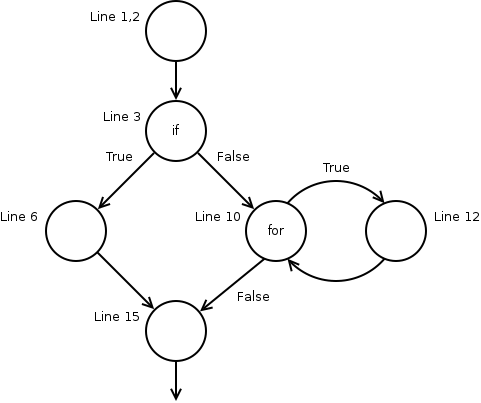
\includegraphics[scale=0.4]{state_transition.png}
\end{frame}

\begin{frame}
    \frametitle{All-Uses Coverage}
    \centering
    \begin{tabular}{ l l l }
        Var & du-path & Tests\\ \hline
        n & $\langle1, 3, 10\rangle$ & -1, 1, 2\\
        f & $\langle2, 15\rangle \langle6, 15\rangle \langle12, 15\rangle$ & -1, 2\\
        i & $\langle10\rangle \langle10, 12\rangle$ & 1, 2
    \end{tabular}
\end{frame}


%------------------------------------------------

\begin{frame}
    \frametitle{The End}

    %\Huge{\centerline{The End}}
    \begin{quote}
        ``Testing shows the presence, not the absence of bugs.''
        \raggedleft{--- Edsger W. Dijkstra}
    \end{quote}
\end{frame}

%----------------------------------------------------------------------------------------

\end{document}

